\documentclass[17pt,a4paper]{extarticle}
\usepackage[p,osf]{scholax}
\usepackage{amsfonts,amstext,amsbsy,amsopn,amsmath,eucal,bm,mathrsfs}
% amssymb should not be loaded
\usepackage[cp1252]{inputenc}
%\usepackage[T1]{fontenc}
\usepackage{textcomp}
\usepackage[varqu,varl]{zi4}% inconsolata
\usepackage[scaled=1.075,ncf,vvarbb]{newtxmath}% need to scale up math package % vvarbb selects the STIX version of blackboard bold.
\normalfont
\usepackage[parfill]{parskip}% Begin paragraphs with an empty line rather than an indent
\usepackage{hyperref}
\usepackage{wrapfig} % wrapping figures
\usepackage{graphicx,color}
\usepackage[labelformat=empty]{caption}
\usepackage[caption = false]{subfig}
\usepackage{fancyhdr} % For headers and footers
\usepackage[landscape]{geometry}
\usepackage{enumitem}
\usepackage{linguex}
\usepackage[capitalise]{cleveref}
\usepackage[most]{tcolorbox}
\usepackage{mdframed} % Add easy frames to paragraphs
\usepackage{xparse} % Add support for \NewDocumentEnvironment

\providecommand{\promed}[1]{{\mathbb{E}}\left\lbrace #1\right\rbrace}% operador de promedio
\providecommand{\var}[1]{{\ensuremath{var}}\{#1\}}
\providecommand{\ve}[1]{{\boldsymbol {#1}}} %
\providecommand{\mat}[1]{{\pmb {#1}}} 
\providecommand{\Real}{\mathbb{R}}\newcommand{\N}{\mathbb{N}}
%%
\definecolor{light-gray}{gray}{0.96}
\definecolor{light-red}{rgb}{0.82, 0.1, 0.26}
\definecolor{light-smoke}{rgb}{0.96,0.96,0.93} 
\definecolor{light-olive}{rgb}{0.63,0.57,0.33} 
\definecolor{light-azul}{rgb}{0.25, 0.41, 0.88}
\definecolor{light-red}{rgb}{0.82, 0.1, 0.26}
\newcommand{\gc}[1]{\textcolor{light-azul}{#1}}
\newcommand{\cita}[1]{\textcolor{light-azul}{\boxed{{\Large #1}}}}
\newcommand{\alp}[1]{\textcolor{light-azul}{\texttt{\quad#1}}}


\definecolor{light-gray}{cmyk}{.30,0,0,.67} % define color using xcolor syntax% example

\tcbset{colback=yellow!10!white, colframe=red!50!black, 
	highlight math style= {enhanced, %<-- needed for the ’remember’ options
		colframe=gray,colback=gray!10!white,boxsep=0pt}
}

\newmdenv[ % Define mdframe settings and store as leftrule
linecolor=light-gray,
topline=false,
bottomline=false,
rightline=false,
skipabove=\topsep,
skipbelow=\topsep
]{leftrule}

\NewDocumentEnvironment{example}{O{\textbf{Example:}}} % Define example environment
{\begin{leftrule}\noindent\textcolor{light-gray}{#1}\par}
	{\end{leftrule}}
%%

\sloppy
\makeatletter
\newcommand{\labelpethau}[1]{\texttt{#1}:}
\newlength\normalparindent
\setlength\normalparindent{\parindent}
\newenvironment{pethau}%
{\begin{list}{}%
		{\renewcommand{\makelabel}{\labelpethau}%
			\setlength{\itemindent}{0pt}%
			\setlength{\leftmargin}{0pt}%
			\setlength{\labelwidth}{-1\normalparindent}%
			\addtolength{\topsep}{-0.5\parskip}%
			\listparindent \normalparindent
			\setlength{\parsep}{\parskip}}}%
	{\end{list}}
\makeatother
%%
\geometry{
	a4paper, % Change this if you intend to print on a different paper size, such as letter paper.
	total={210mm,297mm},
	left=20mm,
	right=20mm,
	top=30mm,
	bottom=30mm,
}
\pagestyle{fancy}

%Settings

\title{\courseName}

\lhead{\courseName} % Left header
\chead{} % Center header
\rhead{} % Right header
\lfoot{} % Left footer
\cfoot{\thepage} % Center footer
\rfoot{} % Right footer

\renewcommand{\headrulewidth}{0.5pt}
\renewcommand{\footrulewidth}{0.3pt}
\renewcommand*\rmdefault{ppl} %Set font
\usepackage{trace}
\usepackage{lineno}

\newcommand{\courseName}{\emph{Spectral~Sensing~for~Wireless Communication~Monitoring}} % Insert course name here
\begin{document}
\maketitle
\thispagestyle{fancy}
\clearpage\newpage
\section{Spectral~Sensing}
\begin{itemize}
	\item Signal Detection

	\item Signal Classification
	
	\item Channel-State Estimation
% 	Adaptation and Optimization:
%Cognitive radio systems continuously adapt their filtering and demodulation parameters based on real-time spectrum sensing feedback to optimize performance.
%Adaptive algorithms may adjust filter bandwidths, demodulation schemes, and other parameters to maximize throughput, minimize interference, and maintain reliable communication under changing channel conditions.
	\item Decision Making
	
	\item Monitoring and System Management
\end{itemize}
\clearpage\newpage
\subsection{Signal~Detection}
\begin{itemize}
	\item Data Collection and Assembly:
	\begin{itemize}
		\item Signal Reception Arrangement
		\item Sampling and  ADC Conversion
		\item Data Storage
 \end{itemize}
 \item Signal Conditioning
 \begin{itemize}
 		
\item Data cleaning and anomaly detection

\item Narrowband Filtering and demodulation

\item Wideband Signal Decimation
 	
 \end{itemize}
\item Energy calculation
\begin{itemize}
	\item Power Estimation and frequency scanning
	\item Noise (SNR) Estimation 
	\item Thresholding 
\end{itemize}
\end{itemize}
\clearpage\newpage
\subsubsection{Data Collection and Assembly}
Acquisition, down/sampling, storage, and preparation of sample sets holding primary information.

\begin{itemize}
\item Enhanced signal reception  
\begin{itemize}
\item
Diversity Antennas for reducing the impact of fading and shadowing:  spatial diversity (using multiple antennas at different locations), polarization diversity (utilizing antennas with different polarization orientations), frequency diversity, and pattern diversity (employing antennas with different radiation patterns).
\item 
Enhanced Detection Sensitivity: By combining signals from multiple antennas, diversity combining techniques such as selection diversity, maximal ratio combining (MRC), or equal gain combining (EGC) can be employed to improve the detection sensitivity of spectrum sensing.
 \item  
Multisensor Sensor Synchronization. Implementing diversity antennas adds complexity to the cognitive radio system, including hardware requirements and signal processing algorithms.
\end{itemize}
\item Sampling and  ADC conversion

Nyquist sampling

Oversampling to improve resolution

Data Compression and Undersampling to feed NN estimators: sigma-delta modulation

Trade-offs between ADC performance parameters (including cost, power consumption, and size)  evaluated based on the specific requirements and constraints of the cognitive radio system.
\item Data Storage

Real-time analysis

Off-line training and validation

Data Retention Policies dictated by regulatory requirements, operational needs, or privacy considerations.

Data anonymization or encryption to protect sensitive information and ensure compliance with privacy regulations.

Data storage infrastructure for spectrum sensing applications may include local storage on cognitive radio devices, networked storage systems, or cloud-based storage solutions.
\end{itemize}
\clearpage\newpage
\subsubsection{Signal Conditioning}
\begin{itemize}
\item Data cleaning and anomaly detection

\item Narrow-band Filtering  and demodulation

Narrow-band band pass filtering and adaptive filtering to isolate specific signals or frequency bands of interest while suppressing noise and interference, improving the signal-to-noise ratio (SNR) of the desired signals.



Demodulation involves extracting the original information carried by modulated signals, such as voice, data, or multimedia content.

\item Wideband Signal Decimation

Channelization, filter banks, and multichannel sensing
 
Software-defined filters: Filtering implementation on software-defined radio (SDR) platforms  (processing power, flexibility, cost, and power consumption).

\end{itemize}

\clearpage\newpage
\subsubsection{Signal Presence Detection} 
\begin{linenomath*} 
	\begin{align*}	
		\textrm{Channel~Model}:\quad & \ve{y}= \ve{x} + \ve{\eta},\\
		&\ve{y}=[y_0,y_1,\ldots,y_{K-1}]^{\top},\; 	\ve{x}=[x_0,x_1,\ldots,x_{K-1}]^{\top}\\
		\textrm{Hypothesis}:\quad &\\
		\textrm{Signal~Absence , }H_0 \to \alpha= 0:\quad &y_k = \eta_k,\quad \textrm{}\\
		\textrm{Signal~Presence, }H_1 \to \alpha= 1:\quad &y_k= \alpha x_k + \eta_k; \quad\forall k\in[0,K-1] 
	\end{align*}
\end{linenomath*}
where $x_i$ is a given signal with known shape, $\eta_k$ is White Gaussian Noise having a known variance $\sigma^{2}_\eta$, and $\alpha{\in}\{0,1\}$ is the unknown constant to be estimated.
\begin{linenomath*} 
	\begin{align*}
		&\textrm{ Maximum Likelihood (ML) ratio}\\
		\Lambda ( \ve{y}|\hat{\alpha}) &=
		\frac{P( \ve{y}|\hat{\alpha})}{P( \ve{y})} 
		 > \gamma\textrm{ -- threshold}\\
		 P(\ve{y}|\hat{\alpha})&=\frac{1}{(2\pi \sigma^{2}_{\eta})^{K/2}}\exp\left(-\frac{1}{2\sigma^{2}_{\eta}}\big(\ve{y}-\alpha\ve{x}\big)^{\top}\big(\ve{y}-\alpha\ve{x}\big)\right)\\
		 P(\ve{y})&=\frac{1}{(2\pi \sigma^{2}_{\eta})^{K/2}}\exp\left(-\frac{1}{2\sigma^{2}_{\eta}} \ve{y} ^{\top} \ve{y} \right)
	\end{align*}
\end{linenomath*}

The estimation of $\hat{\alpha}$ the ML rule is as follows:
\begin{linenomath*} 
	\begin{align*}
		\frac{\partial }{\partial \alpha}	\Lambda ( \ve{y}|\hat{\alpha})&=0 	\\
		\frac{\partial }{\partial \alpha}\ln P(\ve{y}|\hat{\alpha})&=0 	\\
		\frac{\partial }{\partial \alpha}(\ve{y}^{2}-2\alpha\ve{x}\ve{y}+\alpha^{2}\ve{y}^{2})&=0\\	
		-2 \ve{x}\ve{y}+\alpha \ve{y}^{2}&=0
	\end{align*}
\end{linenomath*}

So, the optimal value yields the estimation value for $\hat{\alpha}$:
\begin{linenomath*} 
	\begin{align*}
		 {\hat{\alpha}}& ={\frac{\ve{y}^{\top}\ve{x}}{\ve{x}^{\top}\ve{x}}}\\
		 &= \frac{1}{\|\ve{x}\|}{\ve{y}^{\top}\ve{x}}\\
		 \\
		 {\hat{\alpha}}&=	
		 \frac{\sum\limits_{\forall k \in K}{ y_kx_k}}{\sum\limits_{\forall k \in K}{x^{2}_k}}
	\end{align*}
\end{linenomath*}

Now, we calculate the log of ML 
inequality, $\Lambda (\ve{y}|\hat{\alpha}) >\gamma$:
\begin{linenomath*} 
	\begin{align*}
		-\frac{1}{2\sigma^{2}_{\eta}}\sum_{\forall k \in K}{(-2\hat{\alpha}x_ky_k +\hat{\alpha}^{2}\ve{x}^{2})}&>\ln \gamma
	\end{align*}
\end{linenomath*}
Replacing $ {\alpha}$ by its estimate of $\hat{\alpha}$:
\begin{linenomath*} 
	\begin{align*}
		-\frac{1}{2\sigma^{2}_{\eta}}\left(-2\hat{\alpha}\hat{\alpha}\sum_{\forall k \in K}{x^{2}_k +\hat{\alpha}^{2}}\sum_{\forall k \in K}{x^{2}_k}\right)&>\ln\gamma
	\end{align*}
\end{linenomath*}
Therefore, each hypothesis $H_i$ about the signal holds, as below:
\begin{linenomath*} 
	\begin{align*}
		\hat{\alpha}^{2}\quad&\substack{H_1\\>\\<\\H_0}\quad\frac{2\sigma^{2}_{\eta}\ln\gamma}{\sum_{\forall k \in K}{x^{2}_k}}\\
		\sum_{\forall k \in K}{x^{2}_ky^{2}_k}\quad& \substack{H_1\\>\\<\\H_0}\quad 2\sigma^{2}_{\eta}\ln\gamma\\
		 {\big |\sum_{\forall k \in K}{x _ky _k}\big |}\quad& \substack{H_1\\>\\<\\H_0}\quad {\sqrt{2\sigma^{2}_{\eta}\ln\gamma}}, \,\ve{x} \textrm{ \gc{is not available practically!} }
	\end{align*}
\end{linenomath*}
\clearpage\newpage
\paragraph{Energy calculation.}
 By the law of large numbers (that is, making $K_{\alpha}{\to} \infty$), we have:
\begin{linenomath*} 
	\begin{align*}
		\mathcal{N}(\mu_1,\sigma_{\eta})+\mathcal{N}(\mu_2,\sigma_{\eta}) &\to \mathcal{N}((\mu_1+\mu_2)/2,\sigma_{\eta})\\
		\Rightarrow\mathcal{N}(0,\sigma_{\eta})+\mathcal{N}(\mu_2,\sigma_{\eta}) &= \mathcal{N}(\mu_2/2,\sigma_{\eta})\\
		\\
		\textrm{therefore, }\quad{\hat{\alpha}}&\simeq 2 \sum_{\forall k \in K_{\alpha}}{y_k}
	\end{align*}
\end{linenomath*}

\textit{Detection of a zero-mean Gaussian signal and known variance:} 
\begin{linenomath*} 
	\begin{align*}	
		H_0:\quad y_k &= \eta_k,\quad \eta_k\sim \mathcal{N}_{\ve{\eta}}(0,\sigma_{\eta})\\
		H_1:\quad y_k &= \alpha x_k + x_k; \quad x_k\sim \mathcal{N}_{\ve{x}}(0,\sigma_{x})\\
		&\quad\textrm{s.t.: } \sigma^{2}_{x} > \sigma^{2}_{\eta},\textrm{ high SNR condition}
	\end{align*}
\end{linenomath*}

Therefore, it holds that:
\begin{linenomath*} 
	\begin{align*}
		\sigma^{2}_y&=\sigma^{2}_{a} + \sigma^{2}_{\eta},\\ 
		\Rightarrow\Lambda (y|\hat{\alpha}) &= \frac{P(\ve{y}|\hat{\alpha})}{P(\ve{y}|0)}   	= \frac{\mathcal{N}_{y}(0,\sigma_{y})}
		{\mathcal{N}_{\eta}(0,\sigma_{\eta})}\substack{H_1\\>\\<\\H_0} \gamma 
	\end{align*}
\end{linenomath*}

\begin{wrapfigure}{r}{.48\textwidth}
	\centering
	\resizebox{.45\textwidth}{!}{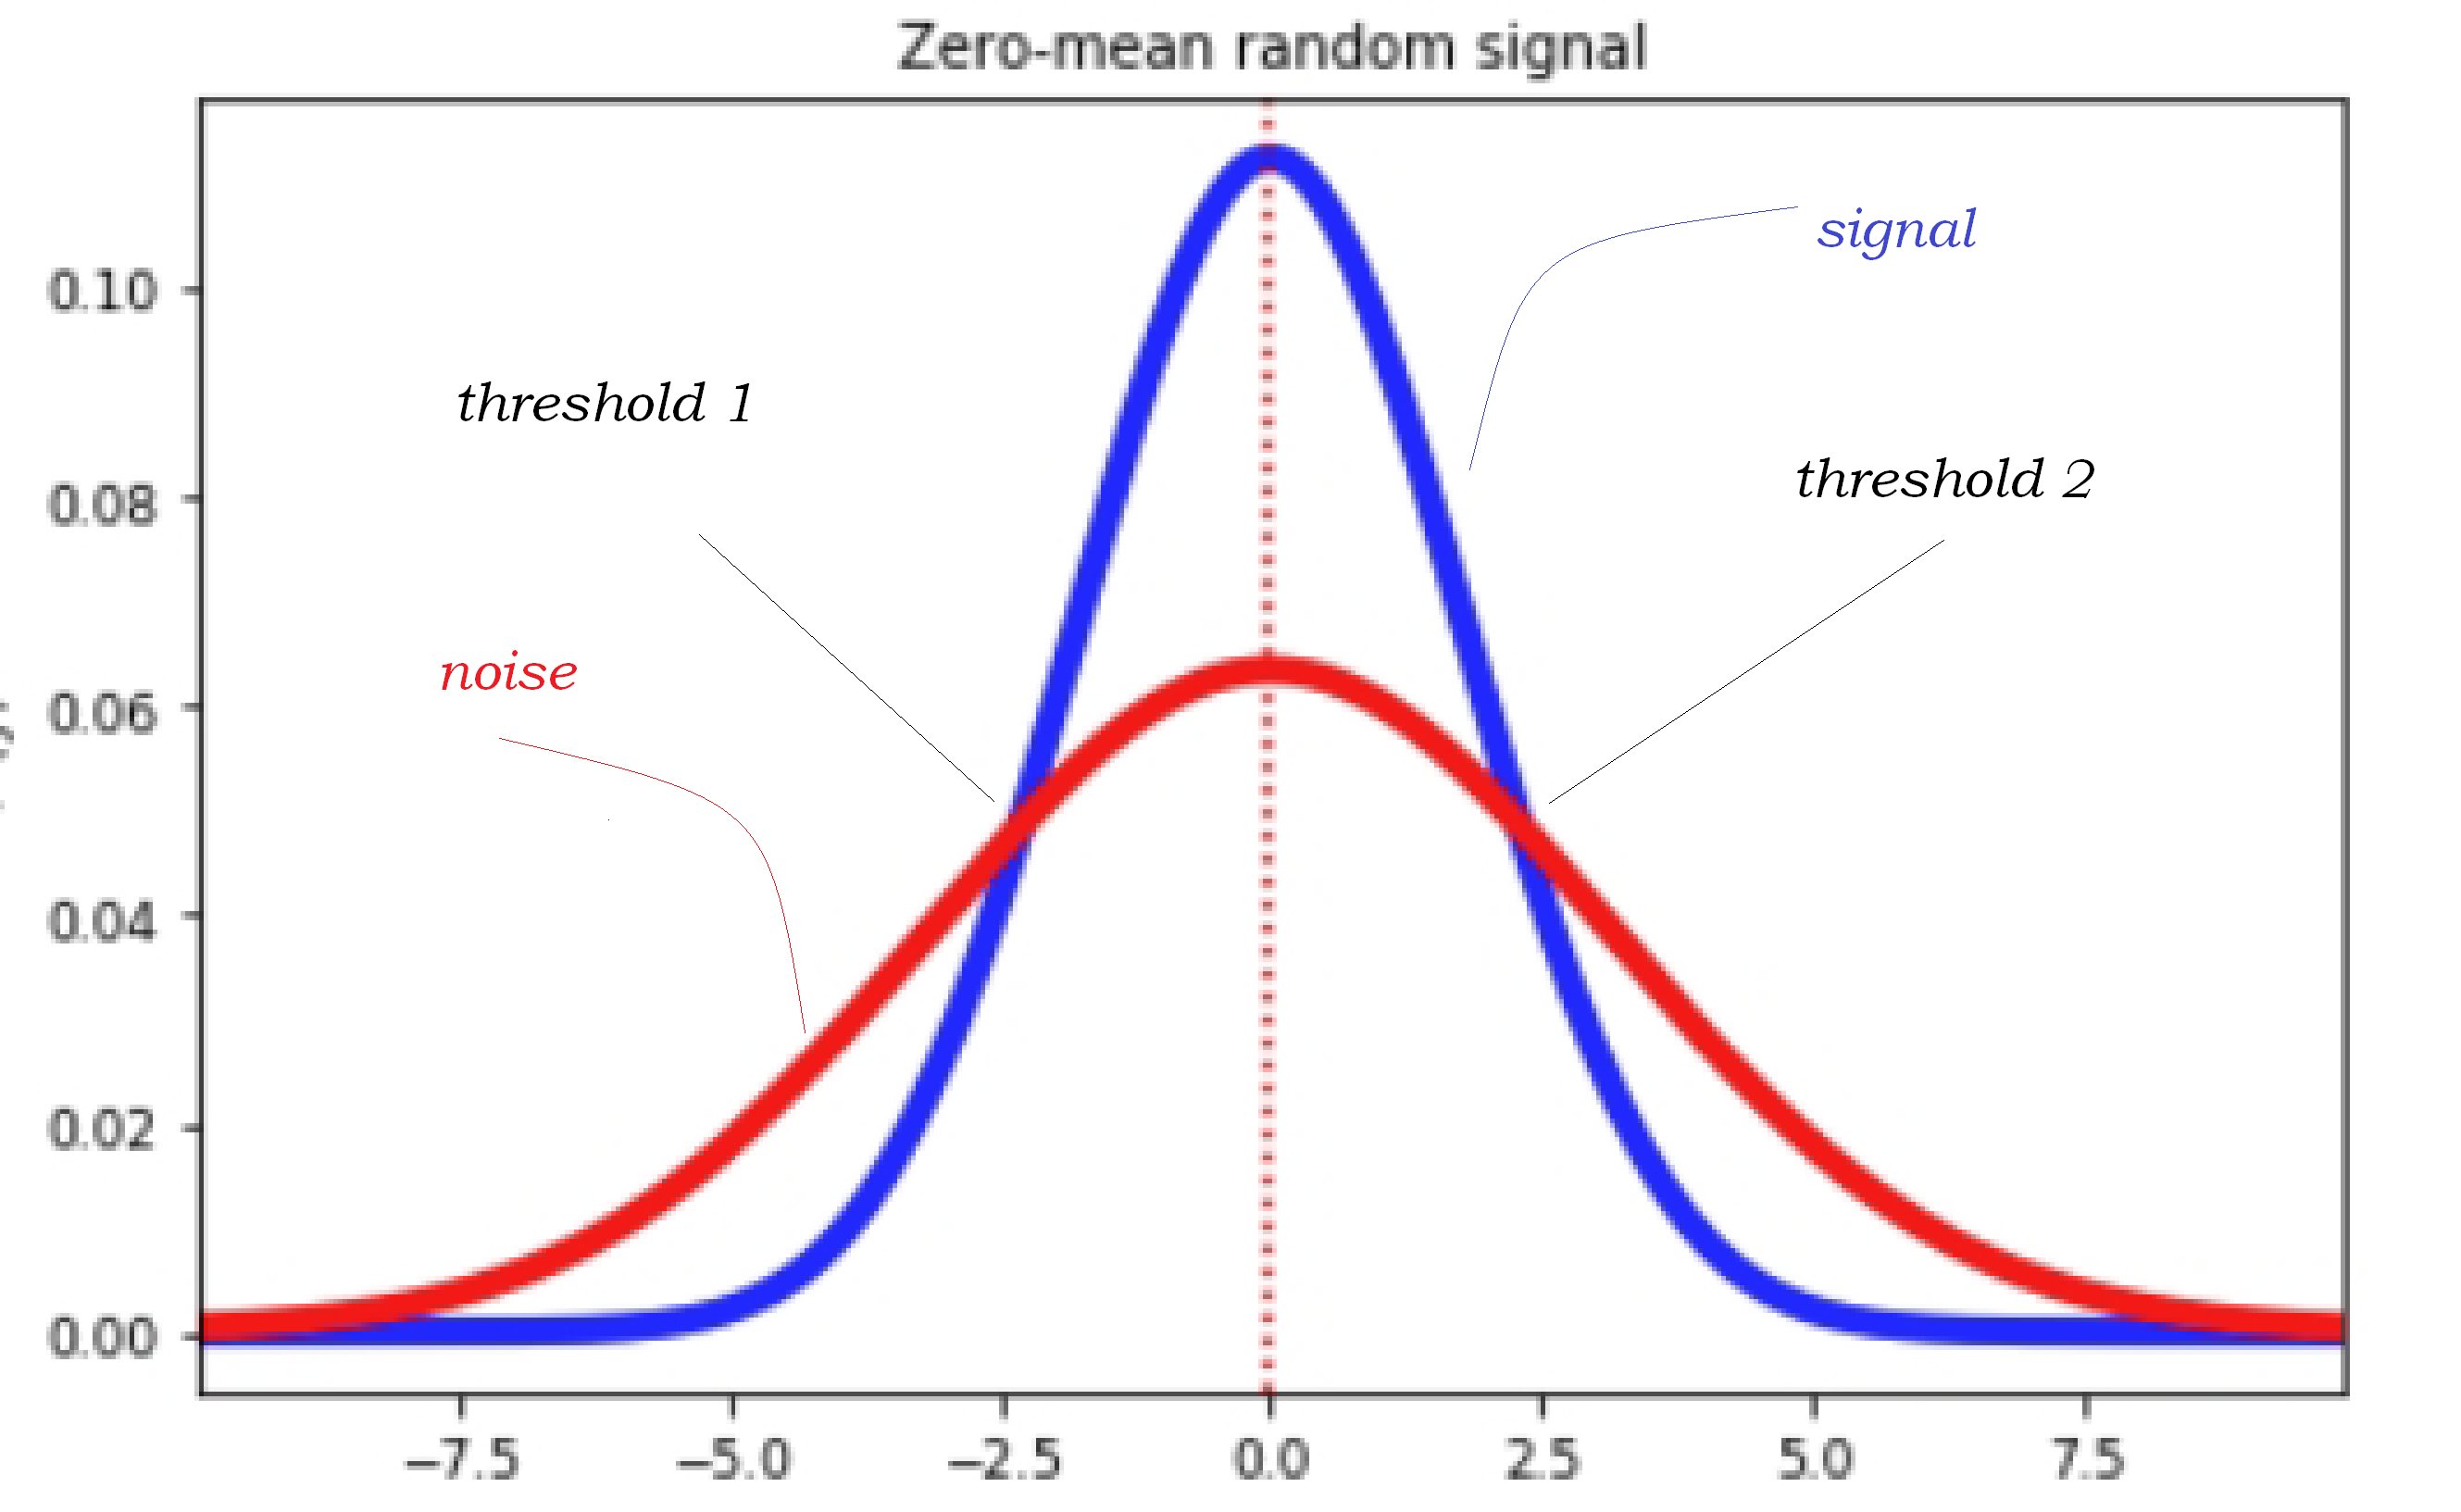
\includegraphics{Figures/EnergySignalSignal}}\\
	\caption{Gaussian signal plus noise with high SNR}\label{Fig:DiagRxOptDig}
\end{wrapfigure}

From ML rule, after some simplifications, we have:
\begin{linenomath*} 
	\begin{align*}
		\sum_{\forall k\in K}y^{2}_k\big( \frac{1}{\sigma^{2}_{\eta}} - \frac{1}{\sigma^{2}_{y}}\big)&= K \ln (\sigma^{2}_{y}/\sigma^{2}_{\eta}+\gamma)\\
		\\
		\sum_{\forall k\in K}y^{2}_k&=K m_{2y}\\
		&=\big( \frac{1}{\sigma^{2}_{\eta}} - \frac{1}{\sigma^{2}_{y}}\big)^{-1} K \ln (\sigma^{2}_{y}/\sigma^{2}_{\eta}+\gamma)\\
		\\
		 {m_{2y}}&= {\big( \frac{1}{\sigma^{2}_{\eta}} - \frac{1}{\sigma^{2}_{y}}\big)^{-1} \ln (\sigma^{2}_{y}/\sigma^{2}_{\eta} )},\qquad \textrm{making }\gamma=1\\
		 & \simeq \sigma^{2}_{\eta} \ln (\sigma^{2}_{y}/\sigma^{2}_{\eta} ), \; \sigma^{2}_{y}/\sigma^{2}_{\eta}\gg 1
	\end{align*}
\end{linenomath*}
\end{document}


Internet of Things (IoT) Development

Amateur Radio
